\nonstopmode  % to allow pdflatex to compile even if errors are raised (e.g. missing figures)

\documentclass[10pt]{article}

\usepackage{amsmath}
\usepackage{amssymb}
\usepackage{bm}
\usepackage{graphicx}
% \graphicspath{{./figures/}} % save all figures in the same directory
\usepackage{color} 
\usepackage{hyperref}
\usepackage{parskip}
\setlength{\parindent}{0pt}

% Text layout
\topmargin 0.0cm
\oddsidemargin 0.5cm
\evensidemargin 0.5cm
\textwidth 16cm 
\textheight 21cm

%% PLEASE INCLUDE ALL MACROS BELOW
\newcommand{\etal}{\textit{et al.}} % use as "\etal{}" in citations
%\newcommand{\Prob}{\mathbb{P}} % symbol for proba
\newcommand{\Prd}{\mathsf{P}} % symbol for discrete proba
\newcommand{\Exp}{\mathbb{E}} % symbol for expectation
\newcommand{\Var}{\mathbb{V}} % symbol for variance
\newcommand{\Cov}{\mathbb{C}} % symbol for covariance
\newcommand{\Norm}{{\mathcal{N}}} % symbol for Normal distribution
\newcommand{\BF}{{\text{BF}}} % symbol for Bayes factor
\newcommand{\Lik}{{\mathcal{L}}} % symbol for 

\begin{document}
\title{Exact Procedure: With Z stats}
\author{Sarah Urbut}
\date{\today}
\maketitle

\begin{itemize}

First, I load the 16,069 x 44 matrix of maximum z statistics statistics into memory. I had previously computed the SFA decomposition on this matrix using 5 factors on the $\textbf{PPS Cluster}$. The steps that follow were run on the $\textbf{Midway Cluster}.

\begin{verbatim}

z.stat <- read.table("maxz.txt")
lambda.mat=as.matrix(read.table("zsfa_lambda.out"))
factor.mat=as.matrix(read.table("zsfa_F.out"))
\end{verbatim}



\section{ Deconvolution Step}

For a given $\omega_{l}$, we specify 4 `types' of $RxR$ prior covariance matrices $U_{k,l}$.
\begin{enumerate}

\item $U_{k=1,l}$ = $\omega_l$ $\mathbf{I}_{R}$

\item $U_{k=2,l}$ = $\omega_l$X_{z}$ The (naively) estimated tissue covariance matrix as estimated from the column-centered J \times R$ matrix of $Z$ statistics, $Z_{center}$: $\frac{1}{J}$ $Z_{center}$^{t}$ $Z_{center}$

\item $U_{k=3,l}$ = $\omega_l$ $\frac{1}{J}$ $V_{1...p}$ $d^{2}_{1...p}$   $V^{t}_{1..p}$ is the rank $p$ eigenvector approximation of the tissue covariance matrices, i.e., the sum of the first $p$ eigenvector approximations, where $\pcv_{1...p}$  represent the eigenvectors of the covariance matrix of tissues and $\pcd_{1...p}$ are the first $p$ eigenvalues.

\item $U_{k=4:4+Q,l}$ = $\frac{1}{J}(($\Lambda\mathbf{F})^{t} \Lambda \mathbf{F})_{q}$ corresponding to the $q_{th}$ sparse factor representation of the tissue covariance matrix %(not the sum of the first $q$, as above)

\item $U_{k=4+Q+1,l}$ = $\frac{1}{J}$ ($\($\Lambda \mathbf{F})^{t} \Lambda \mathbf{F}$ is the sparse factor representation of the tissue covariance matrix, estimated using all $q$ factors.

\end{enumerate}


To retrieve a 'denoised' or 'deconvoluted' estimate of the non-single rank dimensional reduction matrices, I then perform deconvolution.em which initializes the EM algorithm with  the matrices specified in (2), (3) and (5). The final results of this iterative procedure preserves the rank of the initialization matrix, and allows us to use the 'true' effect component as missing data in deconvoluting the prior covariance matrices.

In brief, this is how the deconvolution.em algorithm works.

\begin{enumerate}
\item Produce a 2 element list of initialization parameters containing the initial covariance matrices and a vector of their initial weights, $\mathbf{\pi}$. Critically, this vector $\mathbf{\pi}$ will need to be recomputed when we add these deconvoluted estimates to the full set of covariance matrices.

%\item Choose `zstrong' as the top $permsnp$ gene-pairs  and 'learn' the denoised covariance matrix from this choice. In practice, we use the maximum snp per gene, thus learning from the full set of 16,069 genes.
\item Return a list with the denoised covariance matrix and corresponding mixture weights.
\end {enumerate}

From extensive investigation with testing and training data, I found that using a rank 3 SVD approximation for the matrix in (5) as well as the rank 5 SFA approximation and the empirical covariance matrix maximized the likelihood of a test data set. 

After loading the correct package (i.e., $library('ExtremeDeconvolution')$)
\begin{verbatim}
max.step=deconvolution.em.with.bovy(t.stat=t.stat,factor.mat=factor.mat,lambda.mat=lambda.mat,K=3,P=3)
\end{verbatim}
%deconvolution.em <- function(t.stat,factor.mat,lambda.mat,K,P,permsnp=10000){##note here that we have let t.stat = z.stat
%  init.cov=init.covmat(t.stat=t.stat,factor.mat = factor.mat,lambda.mat = lambda.mat,K=K,P=P)
%  pi=rep(1/K,K)
%  R=ncol(t.stat)
%  
%  par.init=list(true.covs=init.cov,pi=rep(1/K,K))
%  par.init.unlist=unlist(par.init)
%  
%  
%  maxes=apply(t.stat,1,function(x){mean(abs(x))})##takes the strongest t statistics
%  a=cbind(t.stat,maxes)
%  t=a[order(a$maxes,decreasing=TRUE),-45]
%  t.strong=t[1:permsnp,]
%  s.strong=matrix(rep(1,R*nrow(t.strong)),nrow=nrow(t.strong))
%
%  s=squarem(par=par.init.unlist,b.j.hat=t.strong,se.j.hat=s.strong,fixptfn=fixpoint.cov, objfn=negpenlogliksarah)
%  max.step.unlist=s$par
%  dim.true.covs=c(K,R,R)
%  pi.length=length(pi)
%  max.step = list(true.covs = array(max.step.unlist[1:prod(dim.true.covs)], dim = dim.true.covs), pi = max.step.unlist[(prod(dim.true.covs)+1):(prod(dim.true.covs)+pi.length)])
%  return(max.step)
%}


\section{Generation of List of Covariance Matirce}
I then use these three non single-rank covariance matrix in place of our original choice of the empirical covariance matrix, SFA and SVD approximations to create a KxL list of covariance matrices. The function $\textbf{compute.hm.covmat}$ chooses an 'L' element grid according to the range of effect sizes present in the initial 16,069 x 44 matrix of strong Z statistics. 
Here, I also used the Identity (K=1), 5 single-rank SFA factors (K=4-9), and the 44+1 eqtlbma.lite configurations (K=10:54). This is 54 matrices, and in this data set, $\textbf{autoselect.mixgrid}$ chose a grid with 22 omegas for a total of 1188 covariance matrices.

\begin{verbatim}
covmat=compute.hm.covmat.all.max.step(z.stat,v.j,Q=5,lambda.mat,
A="filename",factor.mat,max.step=max.step)

\end{verbatim}

$\textbf{covmat}$ is thus a list of 1188 covariance matrices.


\section{Mixture Weights}
We now need to compute the mixture weights hierarchically. I use  a randomly chosen set of 20000 gene snp pairs from the matrix QTL output to estimate these mixture proportions. This set does not contain the strongest gene-snp pairs, and thus will allow for substantial shrinkage, as a majority of these gene-snp pairs will  have their likelihood maximized at low $\omega$ components.

Here is a visualization of the training data, which you can see is a mixture of mostly small $\hat{\beta}$ and accordingly small Z statistics.

\begin{figure}[h!]
  \caption{Distribution of MLEs}
  \centering
    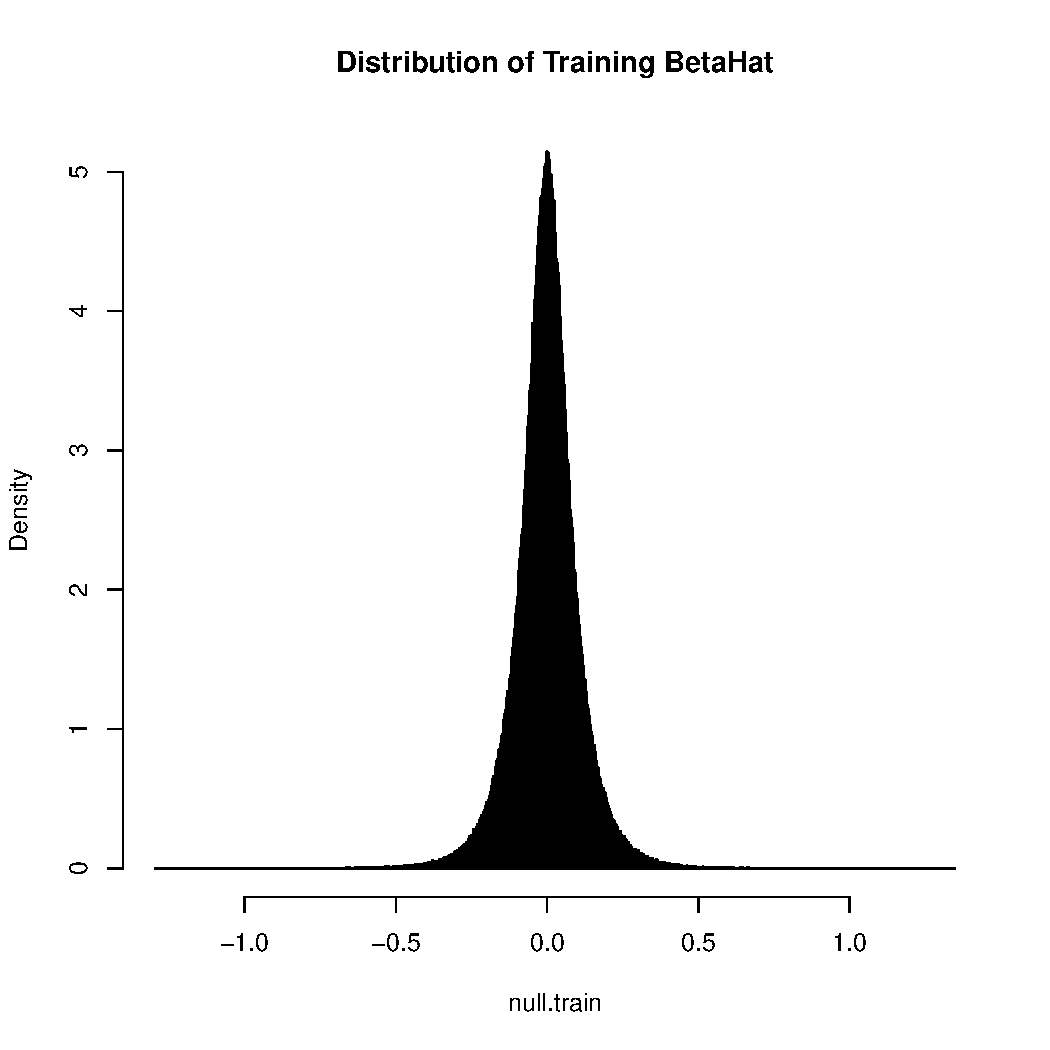
\includegraphics[width=0.5\textwidth]{../Figures/distributionofbhattrain.pdf}
\end{figure}

\begin{verbatim}
compute.hm.train(train.b = train.z,se.train = train.s,covmat = covmat,A="jul3")
\end{verbatim}

$\textbf{compute.hm.train}$ produces an rds object with prior weights, a likelihood matrix, and a pdf of the barplot of these weights.

\section{Posterior Quantities}
Now that I have the estimated mixture weights stored in the vector $\textbf{pis}$. I proceed to the inference step, where I compute the posterior weights and corresponding posterior quantities across all original 16069 gene snp pairs. In brief, the posterior mean, post covariance matrix and tissue specific tail probabilities are computed across all K components for each gene snp pair, and then weighted according to the posterior weights. This is performed in the $\textbf{weightedquants}$ step.


 \begin{verbatim}
weightedquants=lapply(seq(1:nrow(z.stat)),function(j){total.quant.per.snp(j,covmat,b.gp.hat=z.stat,
se.gp.hat = s.j,pis,A,checkpoint = FALSE)})
\end{verbatim}                          
%  all.arrays=post.array.per.snp(j,covmat,b.gp.hat,se.gp.hat)
%  post.means=all.arrays$post.means
%  post.ups=all.arrays$post.ups
%  post.downs=all.arrays$post.downs
%  post.covs=all.arrays$post.covs
%  post.nulls=all.arrays$post.nulls
%  
%  all.mus=total.mean.per.snp(post.weights,post.means)
%  all.ups=total.up.per.snp(post.weights,post.ups)
%  all.downs=total.down.per.snp(post.weights,post.downs )
%  lfsr=t(lfsr.per.snp(all.ups,all.downs))
%  all.covs.partone=total.covs.partone.persnp(post.means,post.covs,post.weights)
%  marginal.var=all.covs.partone-all.mus^2
%
%\end{verbatim}
This will return a set of 6 files containing the JxR matrix of posterior means, marginal variances, tail probabilities, local false sign rates, and the JxK matrix of posterior weights. Checkpoint = FALSE means that the files will be created (rather than simply outputting an object array which contains the posterior quantities.


\section{Testing and Training}

In order to determine the optimal number and rank of the covariance matrices, we divide our data set into a training and test data set, each containing 8000 genes.

In the training set, we proceed as above: choosing the top SNP for each of the 8000 genes, creating a list of covariance matrices through deconvolution and grid selection of these top 'training gene-snp' pairs. 

Then, within the training data, we similarly choose a random set of gene-snp pairs (restricting our analysis to genes contained in the training set. Again, we choose 20,000 random-gene snp pairs and use the EM algorithm to learn the mixture proportions $\pi$  from this data set.

We then use the KxL vector of $\pi$ from the training set to estimate the log likelihood of each data point in the test data set. If our model is 'overfit' to the training data set, than a larger number of covariance matrices may actually decrease the test log-likelihood. 

I found that the K=1188 set of covariance matrices containing the Identity, the denoised empirical covariance matrix, rank 5 SFA approximation and rank 10 SVD approximation as well as 5 single-rank SFA factors and the 45 eqtl.bma.lite configurations maximized this likelihood.


\begin{verbatim}

mdat <- GetSS("max", "/project/mstephens/gtex/analysis/april2015/query/MatrixEQTLSumStats.h5")

ndat <- GetSS("null", "/project/mstephens/gtex/analysis/april2015/query/MatrixEQTLSumStats.h5")

N1 <- 8000
N2 <- 16069
strong.train <- SubsetMatLists(mdat, seq(1, N1))
strong.test <- SubsetMatLists(mdat, seq(N1 + 1, N2))

strong.train.genes <- as.character(lapply(strsplit(rownames(strong.train$beta), "_"), function(x) x[1])) 

strong.test.genes <- as.character(lapply(strsplit(rownames(strong.test$beta), "_"), function(x) x[1]))

null.genes <- as.character(lapply(strsplit(rownames(ndat$beta), "_"), function(x) x[1]))


null.train <- SubsetMatLists(ndat, which(null.genes %in% strong.train.genes))$z[1:20000,]

null.test <- SubsetMatLists(ndat, which(null.genes %in% strong.test.genes))$z[1:20000,]

big.train=strong.train$z
big.test=strong.test$z


max.stepk1=readRDS("maxstep1_train.rds")
max.steprank5=readRDS("maxsteprank5pcfastjul20_train.rds")
max.steprank2=readRDS("maxsteprank2pcfastjul20_train.rds")
#max.steprank10=readRDS("maxsteprank10pc_trainjul20.rds")

max.steprank10=readRDS("trainmaxsteprank10pc.rds")

factor.mat=as.matrix(read.table("../jul3/zsfa_F.out"))
lambda.mat=as.matrix(read.table("../jul3/zsfa_lambda.out"))


z.stat=big.train
rownames(z.stat)=NULL
colnames(z.stat)=NULL
v.j=matrix(rep(1,ncol(z.stat)*nrow(z.stat)),ncol=ncol(z.stat),nrow=nrow(z.stat))



train.z=null.train[1:20000,]
rownames(train.z)=NULL
colnames(train.z)=NULL

train.v=matrix(rep(1,ncol(train.z)*nrow(train.z)),ncol=ncol(train.z),nrow=nrow(train.z))

test.z=null.test
rownames(test.z)=NULL
colnames(test.z)=NULL

##withmaxstepk1"
##compute covarinace matrices on strongest training gene-snp pairs

covmat=compute.hm.covmat(z.stat,v.j,Q=5,lambda.mat,P=2,A="jul21k1",factor.mat,max.step=max.stepk1)

##compute weights on random training set

tim=proc.time()
compute.hm.train(train.b = train.z,se.train = train.v,covmat = covmat,A="jul21k1") ##compute the HM weights on training data
proc.time()-tim

A="jul21k1"
pis=readRDS(paste0("pis",A,".rds"))$pihat

##use training weights to compute test set likelihood
compute.lik.test(test.z,J=nrow(null.test),train.v,covmat,A="jul21k1",pis) 
rm(covmat)
rm(pis)
\end{verbatim}

Here I show the results:



\begin{verbatim}

Run	Likelihood
BMAONLY	-1298672
Rank5withRes	-1283993
Rank2EE	-1277777
NoDecRank5	-1269504
NoDecRank2	-1269442
NoPCNoSFA	-1269277
NOPC	-1268966
K1 Only	-1268622
Rank20	-1268552
Rank10	-1268525
Rank6	-1268520
Rank7	-1268519
Rank12	-1268516
Rank2	-1268322
Rank5NoQ	-1268191
Rank5	-1268102
Rank4	-1268065.997
Rank3maxiter	-1267998.4
rank3 loop 	-1267998.484
Rank3 with single denoise	-1268049.69
rank3ED	-1267887.8

\end{verbatim}

\section{Simulation}
I have also simulated, for each gene snp pair, 100 draws from the multivariate normal distribution characterized by the posterior mean and covariance produced at a component chosen according to its posterior weight (responsibility). For each gene-snp pair, I count the number of simulations in which at least two signs differed. 

\begin{verbatim}
sim.array.generation = function(j,b.j.hat,se.j.hat,covmat,pis,sim){
K=length(covmat)
b.mle=as.vector(t(b.j.hat[j,]))##turn i into a R x 1 vector
V.j.hat=diag(se.j.hat[j,]^2)
lik=lik.func(b.mle,V.j.hat,covmat)
post.weights=lik*pis/sum(lik*pis)
component=apply(rmultinom(sim,1,prob = post.weights),2,function(x){which(x==1)})##choose a component according to responsibility
tinv=lapply(seq(1:sim),function(sim){k=component[sim];solve(covmat[[k]]+V.j.hat)})##generate a list of inverted Ks for all the simulations
b.j.=lapply(seq(1:sim),function(sim){ k=component[sim];post.b.jk.ed.mean(b.mle,tinv=tinv[[sim]],covmat[[k]])})##for each component, compute posterior mean
B.j.=lapply(seq(1:sim),function(sim){ k=component[sim];post.b.jk.ed.cov(tinv=tinv[[sim]],covmat[[k]])})## a list of posterior covariances
simulations=sapply(seq(1:sim),function(x){ 
  dat=mvrnorm(1,mu = b.j.[[x]],Sigma = B.j.[[x]])##for each simulation, generate a multivariate normal according to posterior mean and posterior covariance assigned
   pos=sum(dat>0);neg=sum(dat<0);pos*neg!=0})##for each simulation, ask if they are all one direction; if not, assign1 for heterogeneity
 
return(sum(simulations)/length(simulations)
)}
\end{verbatim}


\end{document}  